% !TEX program = xelatex
\documentclass[12pt,a4paper]{article}

% ---------- Encoding & Language ----------
\usepackage{fontspec}
\usepackage{polyglossia}
\setmainlanguage{greek}
\setotherlanguage{english}
\setmainfont{Times New Roman}
\newfontfamily\greekfont{Times New Roman}

% ---------- Page layout ----------
\usepackage[a4paper,margin=2.5cm]{geometry}
\usepackage{setspace}
\setstretch{1.15}
\usepackage{parskip}

% ---------- Figures / Graphics ----------
\usepackage{graphicx}
\usepackage{float}
\usepackage{subcaption}
\usepackage{booktabs}
\usepackage{enumitem}
\setlist{nosep}

% ---------- Code ----------
\usepackage{listings}
\lstset{basicstyle=\ttfamily\small,frame=single,breaklines=true,tabsize=2,showstringspaces=false}

% ---------- Hyperlinks ----------
\usepackage[hidelinks]{hyperref}

% ---------- TikZ (UML χωρίς ειδικό πακέτο) ----------
\usepackage{tikz}
\usetikzlibrary{arrows.meta,positioning,fit,shapes.geometric}

% ---------- Title ----------
\title{\textbf{Τεχνολογία Λογισμικού: Latex Report - Εργασία Σεπτεμβρίου 2025}}
\author{Λάμπρος Μπουντούλης \\ Επί Πτυχίω - Π2013075}
{}

\begin{document}
\maketitle

\begin{abstract}
Η εργασία παρουσιάζει μια απλή εφαρμογή για εκτέλεση διεργασιών ανάλυσης δεδομένων και Μηχανικής Μάθησης. Ο χρήστης φορτώνει δεδομένα (\texttt{.h5ad} ή \texttt{.mtx+tsv}), ρυθμίζει παραμέτρους και βλέπει άμεσα τρεις βασικές οπτικοποιήσεις: UMAP (διάταξη ομάδων), QC violin (έλεγχος ποιότητας) και heatmap markers (ενδεικτικά γονίδια ανά ομάδα). Η υλοποίηση βασίζεται σε \textit{Scanpy} για το pipeline (QC $\to$ PCA/kNN/UMAP $\to$ Leiden) και σε \textit{Streamlit} για το web UI. Επιπλέον, η χρήση Docker διασφαλίζει ότι η εφαρμογή τρέχει το ίδιο σε κάθε υπολογιστή. Η ροή των διαδικασιών βασίζεται στους κώδικες που δόθηκαν για την εκπόνηση της εργασίας - οι οποίοι αφορούσαν διαφορετικά στάδια αναλύσεψων.
\end{abstract}

\section{Εισαγωγή}
Στόχος είναι η δημιουργία μιας απλής, διαδραστικής εφαρμογής, για γρήγορα αποτελέσματα ανάλυσης δεδομένων. Χωρίς να απαιτούνται γνώσεις προγραμματισμού, ο χρήστης ανεβάζει αρχεία, πατάει Εκτέλεση και παίρνει οπτικοποιήσεις που βοηθούν να ελέγξει την ποιότητα των αναλύσεων. 

\section{Σχεδιασμός της Υλοποίησης}
Η αρχιτεκτονική διαχωρίζει \textbf{λογική ανάλυσης} (\texttt{src/}) από το \textbf{UI} (\texttt{app.py, pages/}). Το \texttt{ScanpyAdapter} εγκιβωτίζει τις κλήσεις στη βιβλιοθήκη, ενώ το \texttt{Pipeline} ενορχηστρώνει τα βήματα.

\subsection*{UML Class Diagram}
\begin{figure}[H]
  \centering
  \begin{tikzpicture}[
    class/.style={draw, rounded corners, align=left, inner sep=2pt, minimum width=4.1cm},
    node distance=1.4cm and 2.0cm,
    rel/.style={-Latex},
  ]
    % Classes
    \node[class] (ui) {\textbf{AppUI (Streamlit)}\\\hrulefill\\\+ render()\\\\+ handle\_inputs()\\\\+ show\_plots()};

    \node[class, below=of ui] (pipe) {\textbf{Pipeline}\\\hrulefill\\\textit{- loader: DataLoader}\\\textit{- pre: Preprocessor}\\\textit{- an: Analyzer}\\\textit{- viz: Visualizer}\\\textit{- exp: Exporter}\\\hrulefill\\\\+ run(params)\\\\+ state()};

    \node[class, right=of pipe] (loader) {\textbf{DataLoader}\\\hrulefill\\\textit{- input\_paths: dict}\\\hrulefill\\\\+ from\_mtx()\\\\+ from\_h5ad()};
    \node[class, above=of loader] (prep) {\textbf{Preprocessor}\\\hrulefill\\\textit{- min\_genes, min\_cells}\\\textit{- n\_top\_genes}\\\hrulefill\\\\+ qc()\\\\+ normalize\_log1p()\\\\+ select\_hvg()};
    \node[class, below=of loader] (an) {\textbf{Analyzer}\\\\\hrulefill\\\\\textit{- n\_pcs}\\\textit{- resolution}\\\hrulefill\\\\+ pca()\\+ neighbors()\\+ umap()\\+ leiden()};

    \node[class, left=of pipe] (viz) {\textbf{Visualizer}\\\\\hrulefill\\\\+ qc\_violin()\\\\+ umap()\\\\+ heatmap()};
    \node[class, below=of viz] (exp) {\textbf{Exporter}\\\hrulefill\\\+ save\_pngs()\\\\+ save\_h5ad()};
    \node[class, above=of viz] (cfg) {\textbf{Config}\\\\hrulefill\\\\textit{- params: dict}\\\hrulefill\\\+ load()\\\\+ to\_dict()};

    % Relations
    \draw[rel] (ui) -- (pipe);

    % Composition from Pipeline to components (filled diamond near Pipeline)
    \draw[rel] (pipe.east) -- node[pos=0.15,shape=diamond,draw,fill=black,inner sep=1.5pt,minimum size=5pt]{} (loader.west);
    \draw[rel] (pipe.east) |- node[pos=0.2,shape=diamond,draw,fill=black,inner sep=1.5pt,minimum size=5pt]{} (prep.south);
    \draw[rel] (pipe.east) |- node[pos=0.2,shape=diamond,draw,fill=black,inner sep=1.5pt,minimum size=5pt]{} (an.north);
    \draw[rel] (pipe.west) -- node[pos=0.85,shape=diamond,draw,fill=black,inner sep=1.5pt,minimum size=5pt]{} (viz.east);
    \draw[rel] (pipe.west) |- node[pos=0.3,shape=diamond,draw,fill=black,inner sep=1.5pt,minimum size=5pt]{} (exp.north);

    % Association to Config
    \draw[rel,dashed] (cfg.east) -- (pipe.west);
  \end{tikzpicture}
  \caption{UML Class Diagram: το Pipeline συνθέτει τα βασικά υποσυστήματα. Το UI καλεί το Pipeline.}
  \label{fig:umlclass}
\end{figure}

\subsection*{UML Use Case Diagram}
\begin{figure}[H]
  \centering
  \begin{tikzpicture}[
    usecase/.style={draw, ellipse, align=center, minimum width=5.2cm, minimum height=1.2cm},
    node distance=7mm and 10mm
  ]
    % Actor
    \coordinate (actor) at (0,0);
    \draw (actor) circle (0.24);
    \draw (0,-0.24) -- (0,-1.0);
    \draw (-0.45,-0.6) -- (0,-0.24) -- (0.45,-0.6);
    \draw (-0.45,-1.4) -- (0,-1.0) -- (0.45,-1.4);
    \node[below=1.7cm] at (actor) {Χρήστης};

    % System boundary
    \node[draw, rounded corners, minimum width=14.5cm, minimum height=6.8cm, right=2.4cm of actor, anchor=west] (sys) {};
    \node at (sys.north) [yshift=-0.3cm] {\textbf{Streamlit scRNA-seq App}};

    % Primary use cases
    \node[usecase, anchor=west] (uc1) at ([xshift=0.9cm,yshift=2.0cm]sys.west) {Φόρτωση Δεδομένων};
    \node[usecase, anchor=west] (uc2) at ([xshift=0.9cm,yshift=0.7cm]sys.west) {Ρύθμιση Παραμέτρων};
    \node[usecase, anchor=west] (uc3) at ([xshift=0.9cm,yshift=-1.1cm]sys.west) {Εκτέλεση Pipeline};
    \node[usecase, anchor=west] (uc4) at ([xshift=6.9cm,yshift=1.9cm]sys.west) {Προβολή Οπτικοποιήσεων};
    \node[usecase, anchor=west] (uc5) at ([xshift=7.3cm,yshift=0.5cm]sys.west) {Εξαγωγή PNG/H5AD};
    \node[usecase, anchor=west] (uc6) at ([xshift=6.9cm,yshift=-0.8cm]sys.west) {Εκτέλεση σε Docker};

    % Included sub-cases
    \node[usecase] (sub1) at ([xshift=2.9cm,yshift=-2.7cm]sys.west) {PCA/kNN/UMAP};
    \node[usecase] (sub2) at ([xshift=9.5cm,yshift=-2.5cm]sys.west) {Ομαδοποίηση (Leiden)};

    % Associations to actor
    \draw (0,-0.8) -- (uc1.west);
    \draw (0,-0.8) -- (uc2.west);
    \draw (0,-0.8) -- (uc3.west);
    \draw (0,-0.8) -- (uc4.west);
    \draw (0,-0.8) -- (uc5.west);
    \draw (0,-0.8) -- (uc6.west);

    % Include relationships (dashed with label)
    \draw[dashed,-Latex] (uc3.south) -- (sub1.north);
    \node at ($(uc3.south)!0.5!(sub1.north)+(-0.2,0)$) {\scriptsize $\langle$include$\rangle$};

    \draw[dashed,-Latex] (uc3.south east) .. controls +(0.8,-0.8) and +(-0.8,0.8) .. (sub2.north west);
    \node at ($(uc3.south east)!0.5!(sub2.north west)+(0.1,-0.1)$) {\scriptsize $\langle$include$\rangle$};
  \end{tikzpicture}
  \caption{UML Use Case: βασικά σενάρια χρήσης και υποπεριπτώσεις με \textit{include}.}
  \label{fig:umluse}
\end{figure}

\section{Ανάλυση της Υλοποίησης με Τεχνικές Λεπτομέρειες}

\subsection{Αρχιτεκτονική λογισμικού}
Η εφαρμογή είναι αρθρωτή:
\begin{itemize}
  \item \textbf{DataLoader}: ανάγνωση δεδομένων \texttt{.h5ad} ή τριάδας \texttt{.mtx + barcodes.tsv + features.tsv} σε \texttt{AnnData}.
  \item \textbf{Preprocessor}: βασικός QC, κανονικοποίηση, \texttt{log1p}, επιλογή γονιδίων υψηλής διακύμανσης (HVGs).
  \item \textbf{Analyzer}: \texttt{PCA} $\to$ \texttt{kNN} $\to$ \texttt{UMAP} $\to$ \texttt{Leiden}.
  \item \textbf{Visualizer}: δημιουργία UMAP, QC violin, heatmap markers και αποθήκευση PNG.
  \item \textbf{Pipeline \& UI}: ενορχήστρωση βημάτων και απλό web UI με \textit{Streamlit}.
\end{itemize}

\subsection{Είσοδος/Έξοδος Δεδομένων}
\paragraph{Μορφές εισόδου.} Υποστηρίζονται:
\begin{enumerate}[leftmargin=*]
  \item \textbf{{.h5ad}}
  \item \textbf{10x MTX set}: \texttt{matrix.mtx.gz}, \texttt{barcodes.tsv.gz}, \texttt{features.tsv.gz}.
\end{enumerate}
\noindent \textit{Συμβατότητα HDF5/συμπίεσης:} για \texttt{.h5ad} με συμπιέσεις όπως blosc/zstd, η φόρτωση γίνεται με εγκατεστημένο \texttt{hdf5plugin}.

\paragraph{Έξοδος.} Παράγονται εικόνες PNG (UMAP, QC, heatmap) στον φάκελο \texttt{figs/} και \texttt{.h5ad} με τα υπολογισμένα αποτελέσματα (π.χ. clusters).

\subsection{Προεπεξεργασία (QC \& φιλτράρισμα)}
\begin{enumerate}[leftmargin=*]
  \item \textbf{Μετρικές QC}
  \item \textbf{Προαιρετικό φιλτράρισμα}
\end{enumerate}

\subsection{Κανονικοποίηση \& μετασχηματισμοί}
\begin{itemize}
  \item \textbf{Normalize}: Κλιμάκωση ανά κύτταρο
  \item \textbf{Log1p}: Σταθεροποίηση διακυμάνσεων
  \item \textbf{HVGs}: Επιλογή x γονιδίων για μείωση θορύβου/διάστασης
  \item \textbf{Scale}: οριοθέτηση τιμών (π.χ. \texttt{max\_value=10}) πριν την PCA.
\end{itemize}

\subsection{Μείωση διάστασης, γράφος \& ομαδοποίηση}
\begin{enumerate}[leftmargin=*]
  \item \textbf{PCA}: συμπύκνωση πληροφορίας.
  \item \textbf{kNN γράφος}: με βάση το PCA.
  \item \textbf{UMAP}: διδιάστατη προβολή για απεικόνιση.
  \item \textbf{Leiden} (\texttt{resolution} ρυθμιζόμενο): υπολογισμός clusters στον γράφο ομοιότητας.
\end{enumerate}

\subsection{Εντοπισμός markers \& εξαγωγές}
Υπολογίζονται διακριτικά γονίδια ανά ομάδα (π.χ. με \texttt{rank\_genes\_groups}) και παράγεται \textbf{heatmap} κορυφαίων markers. Οι εικόνες αποθηκεύονται σε \texttt{figs/} με ανάλυση (π.χ.) 300~dpi.

\subsection{Ενδεικτικός κώδικας}
\begin{lstlisting}[language=Python]
import scanpy as sc

def run_pipeline(adata, n_pcs=30, res=1.0):
    # QC
    adata.var['mt'] = adata.var_names.str.upper().str.startswith(('MT-','MT.'))
    sc.pp.calculate_qc_metrics(adata, qc_vars=['mt'], inplace=True)

    # Normalize + log + HVGs + scale
    sc.pp.normalize_total(adata, target_sum=1e4)
    sc.pp.log1p(adata)
    sc.pp.highly_variable_genes(adata, n_top_genes=2000, subset=True)
    sc.pp.scale(adata, max_value=10)

    # PCA + graph + UMAP + Leiden
    sc.tl.pca(adata)
    sc.pp.neighbors(adata, n_pcs=n_pcs)
    sc.tl.umap(adata, random_state=42)
    sc.tl.leiden(adata, resolution=res)  # σταθερό seed όπου υποστηρίζεται

    return adata
\end{lstlisting}

\subsection{Οπτικοποιήσεις}
\begin{itemize}
  \item \textbf{UMAP}
  \item \textbf{QC violin}
  \item \textbf{Heatmap markers}
\end{itemize}
\noindent \textit{Σημείωση υλοποίησης:} οι συναρτήσεις plotting καλούνται με \texttt{show=False} και οι εικόνες αποθηκεύονται με \texttt{bbox\_inches='tight', dpi=300}.

\subsection{UI \& διαχείριση κατάστασης}
Το \textit{Streamlit} χειρίζεται εισαγωγή αρχείων, παραμέτρους και την κλήση \texttt{run\_pipeline}. Χρησιμοποιείται \texttt{st.session\_state} για να διατηρούνται τα αποτελέσματα μεταξύ ενεργειών (π.χ. αλλαγή παραμέτρων χωρίς επαναφόρτωση αρχείων). Ακριβές caching βαριών βημάτων μπορεί να γίνει με \texttt{@st.cache\_data} (π.χ. για ανάγνωση αρχείων).

\subsection{Απόδοση \& μνήμη}
\begin{itemize}
  \item Χρήση \textbf{αραιών πινάκων} όπου είναι διαθέσιμοι (\texttt{adata.X} CSR) μειώνει μνήμη.
  \item \textbf{HVGs} πριν από PCA/UMAP επιταχύνει σημαντικά τη ροή.
  \item Οι υπολογισμοί στηρίζονται σε \texttt{numba}/\texttt{umap-learn} και \texttt{igraph}/\texttt{leidenalg} όταν υπάρχουν binary wheels.
\end{itemize}

\subsection{Έλεγχος σφαλμάτων \& επικυρώσεις}
\begin{itemize}
  \item Έλεγχος τύπου αρχείων και ύπαρξης απαιτούμενων στηλών (\texttt{barcodes, features}).
  \item Μηνύματα σε μη υποστηριζόμενη συμπίεση \texttt{.h5ad} (πρόταση εγκατάστασης \texttt{hdf5plugin}).
  \item Προστασία από \textit{empty selections} (π.χ. μηδενικά HVGs μετά από αυστηρό φιλτράρισμα).
\end{itemize}

\subsection{Αναπαραγωγιμότητα \& περιβάλλον}
\begin{itemize}
  \item \textbf{Pinned εκδόσεις} στο \texttt{requirements.txt} (π.χ. \texttt{scanpy}, \texttt{anndata}, \texttt{umap-learn}, \texttt{python-igraph}, \texttt{leidenalg}, \texttt{hdf5plugin}, \texttt{streamlit}).
  \item \textbf{Seeds} για \texttt{UMAP}/\texttt{Leiden} όπου υποστηρίζεται.
  \item \textbf{Docker} για ίδιο runtime σε όλα τα συστήματα.
\end{itemize}


\section{Οπτικοποιήσεις Αποτελεσμάτων}
Οι παρακάτω εικόνες παράγονται αυτόματα από την εφαρμογή ως μέρος της τυπικής ροής ανάλυσης.
\begin{figure}[H]
  \centering
  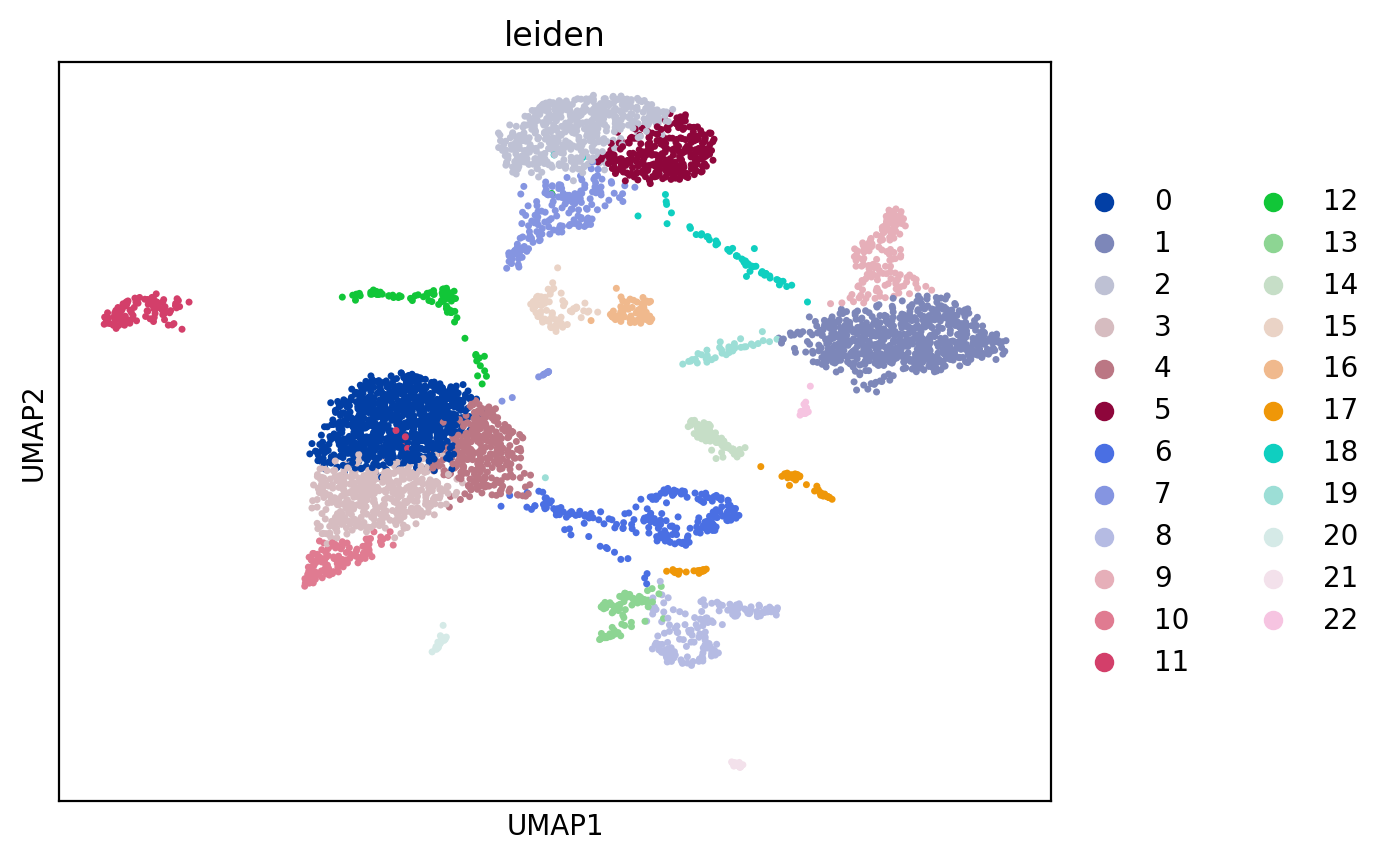
\includegraphics[width=0.85\linewidth]{figs/umap.png}
  \caption{UMAP με χρωματισμό ανά cluster (Leiden).}
  \label{fig:umap}
\end{figure}
\begin{figure}[H]
  \centering
  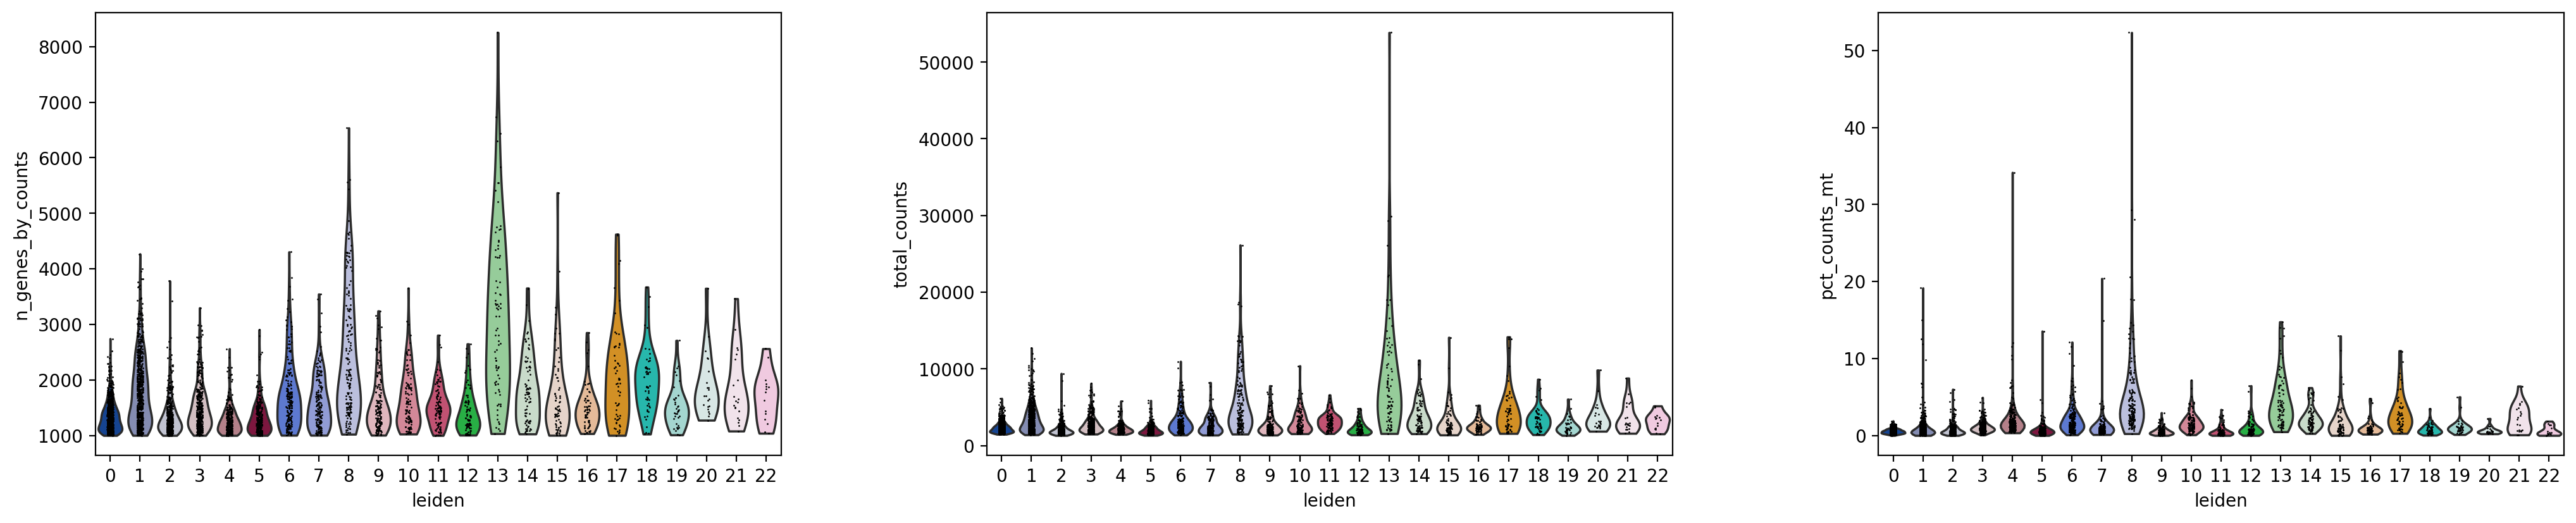
\includegraphics[width=0.85\linewidth]{figs/qc_violin.png}
  \caption{QC violin: genes/cell, counts/cell, ποσοστό μιτοχονδριακών ανά cluster.}
  \label{fig:qc}
\end{figure}
\begin{figure}[H]
  \centering
  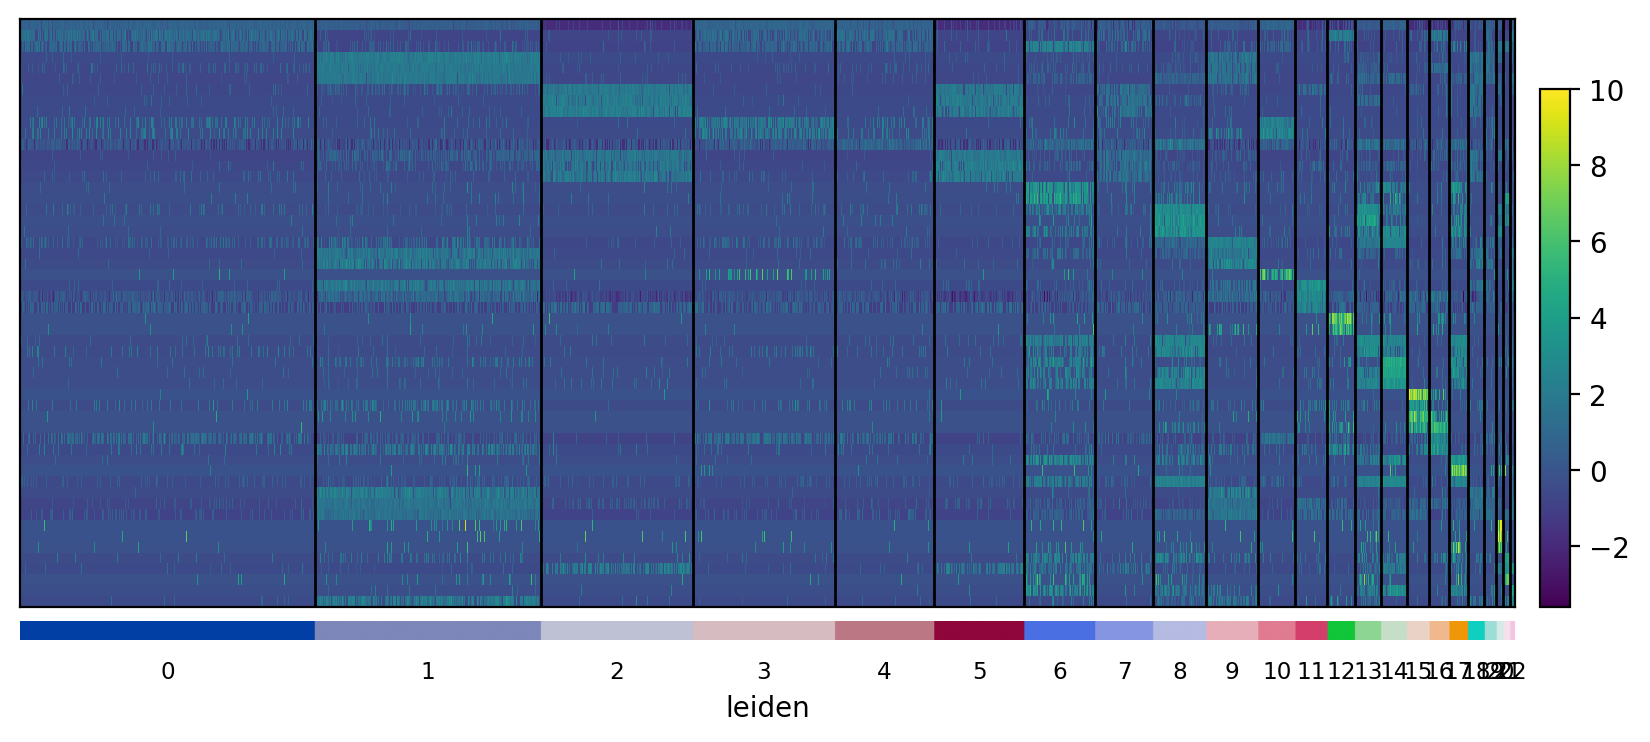
\includegraphics[width=0.85\linewidth]{figs/markers_heatmap.png}
  \caption{Heatmap κορυφαίων markers ανά cluster.}
  \label{fig:heatmap}
\end{figure}

\section{Dockerization της Εφαρμογής}
Ενα Docker image που περιέχει τις εξαρτήσεις και τρέχει το \textit{Streamlit} app.
\subsection*{Dockerfile}
\begin{lstlisting}[language=Dockerfile]
FROM python:3.11-slim
WORKDIR /app
COPY requirements.txt .
RUN pip install --no-cache-dir -r requirements.txt
COPY . .
ENV STREAMLIT_SERVER_HEADLESS=true \
    STREAMLIT_SERVER_PORT=8501 \
    STREAMLIT_BROWSER_GATHER_USAGE_STATS=false
EXPOSE 8501
CMD ["streamlit", "run", "app.py"]
\end{lstlisting}
\subsection*{Build/Run}
\begin{lstlisting}[language=bash]
# Build
docker build -t scrna-app:latest .
# Run (localhost:8501)
docker run --rm -p 8501:8501 -v %cd%/data:/app/data scrna-app:latest
\end{lstlisting}

\\\section{GitHub}
Μπορείτε να βρείτε την εφαρμογή στο GitHub, στο παρακάτω link:
\\https://github.com/p13bounL/TechLog

\end{document}
